\chapter{Rezultate și concluzii}
\section{Evaluarea performanței}
În cadrul evaluării agentului DQN, s-a avut în vedere surprinderea ratei de câștig, a strategiei de cumpărare a proprietăților, rata de faliment, economiile și alți indicatori captați de TournamentManager.

În continuare vom presupune că toate rezultatele au fost obținute în cadrul unui turneu round-robin cu 300 de jocuri per duel, cu 1.000 de runde maxime.

\begin{figure}[H]
    \centering
    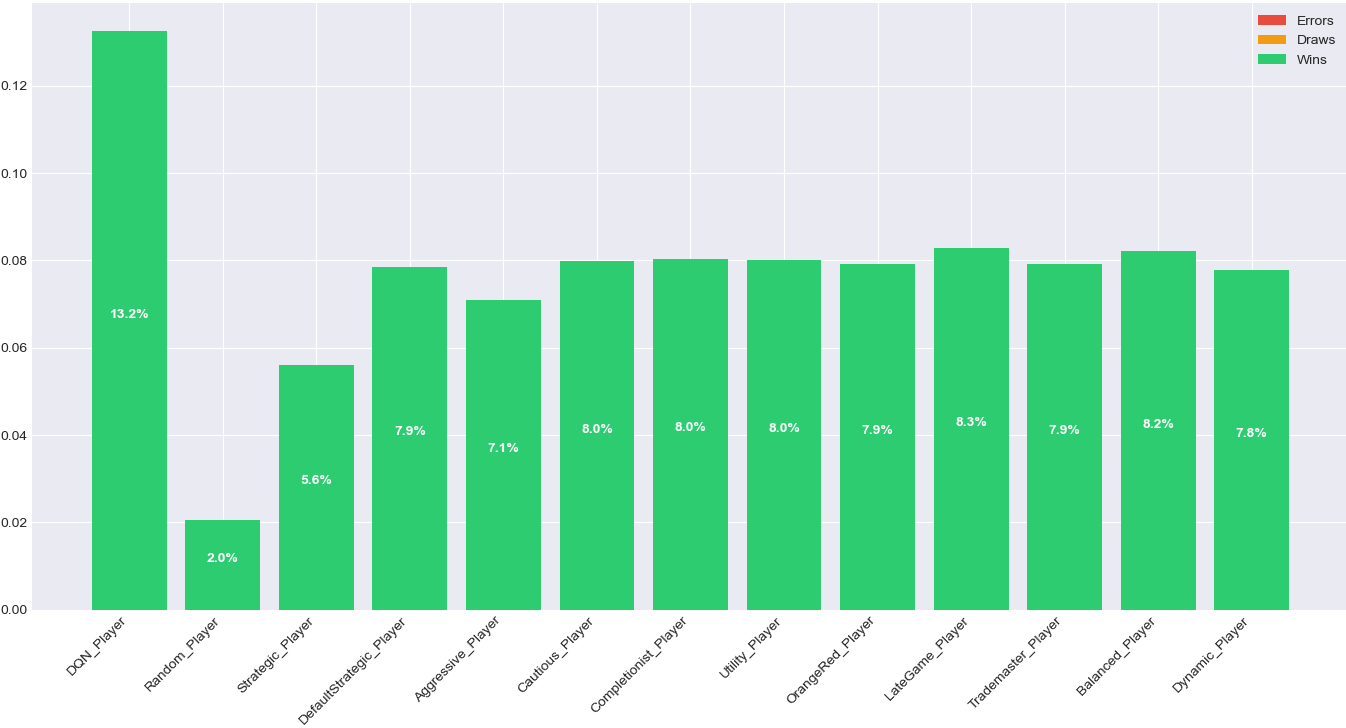
\includegraphics[width=16cm]{images/dqn_tournament_win_rates.png}
    \caption{Rezultatele agentului DQN într-un turneu}
    \label{fig:dqn-tournament-results}
\end{figure}

În figura \ref{fig:dqn-tournament-results}, se poate remarca o prezență dominantă a agentului DQN, acesta reușind să adune o rată de câștig de 13,2\%, cu 5,3\% mai mult față de agentul strategic, demonstrând adaptabilitatea și puterea acestuia de înțelegere a jocului.

Acesta a reușit să aibă o rată de faliment de doar 2\%, media fiind de 6\%, iar în cazul fluidității cash-ului acesta a reușit să adune o avere medie finală de 2321₩, de aproximativ două ori și jumătate mai mult decât media și un cash final mediu de 1865₩, de 4,1 ori mai mult decât media.

În cazul predispoziției de cumpărare, agentul DQN a preferat proprietățile din grupul verde în 30\% din cazuri, urmate de cele galbene (22\%) și albastru închis (18\%), lucru ieșit din comun, având în vedere probabilitatea statistică și rata de retur mediu al investiției. Aceasta se poate datora probabilității mari de câștig, odată securizată latura dintre căsuțele "Du-te la închisoare" și "Start", având cea mai mare chirie percepută în joc, poate lua orice jucător prin surprindere falimentându-l pe neașteptate. Astfel se poate explica și prezența mare a banilor cash la sfârșitul jocului, amintită anterior, jucătorii ajungeau pe aceste căsuțe și nu aveau resursele necesare achitării datoriilor.

Agentul DQN pare să își fi însuțit și un comportament inteligent în privința ipotecării proprietăților în vederea îmbunătățirii proprietăților. Acesta preferă să ipotecheze proprietăți pentru o scurtă durată, în vederea cumpărării caselor, când apreciază că oponentul va ajunge pe proprietățile sale. Ulterior plătirii chiriei, acesta își dezipotechează proprietățile, recuperându-și investiția.

Utilizarea abordării hibride în cazul metodelor distructive, crește rata victoriei cu 3,5\%, în cazul utilizării acesteia pentru toate metodele distructive, fapt ce semnalează prezența unei lipse de antrenare și lipsa înțelegerii depline a consecințelor viitoare.

\begin{figure}[H]
    \centering
    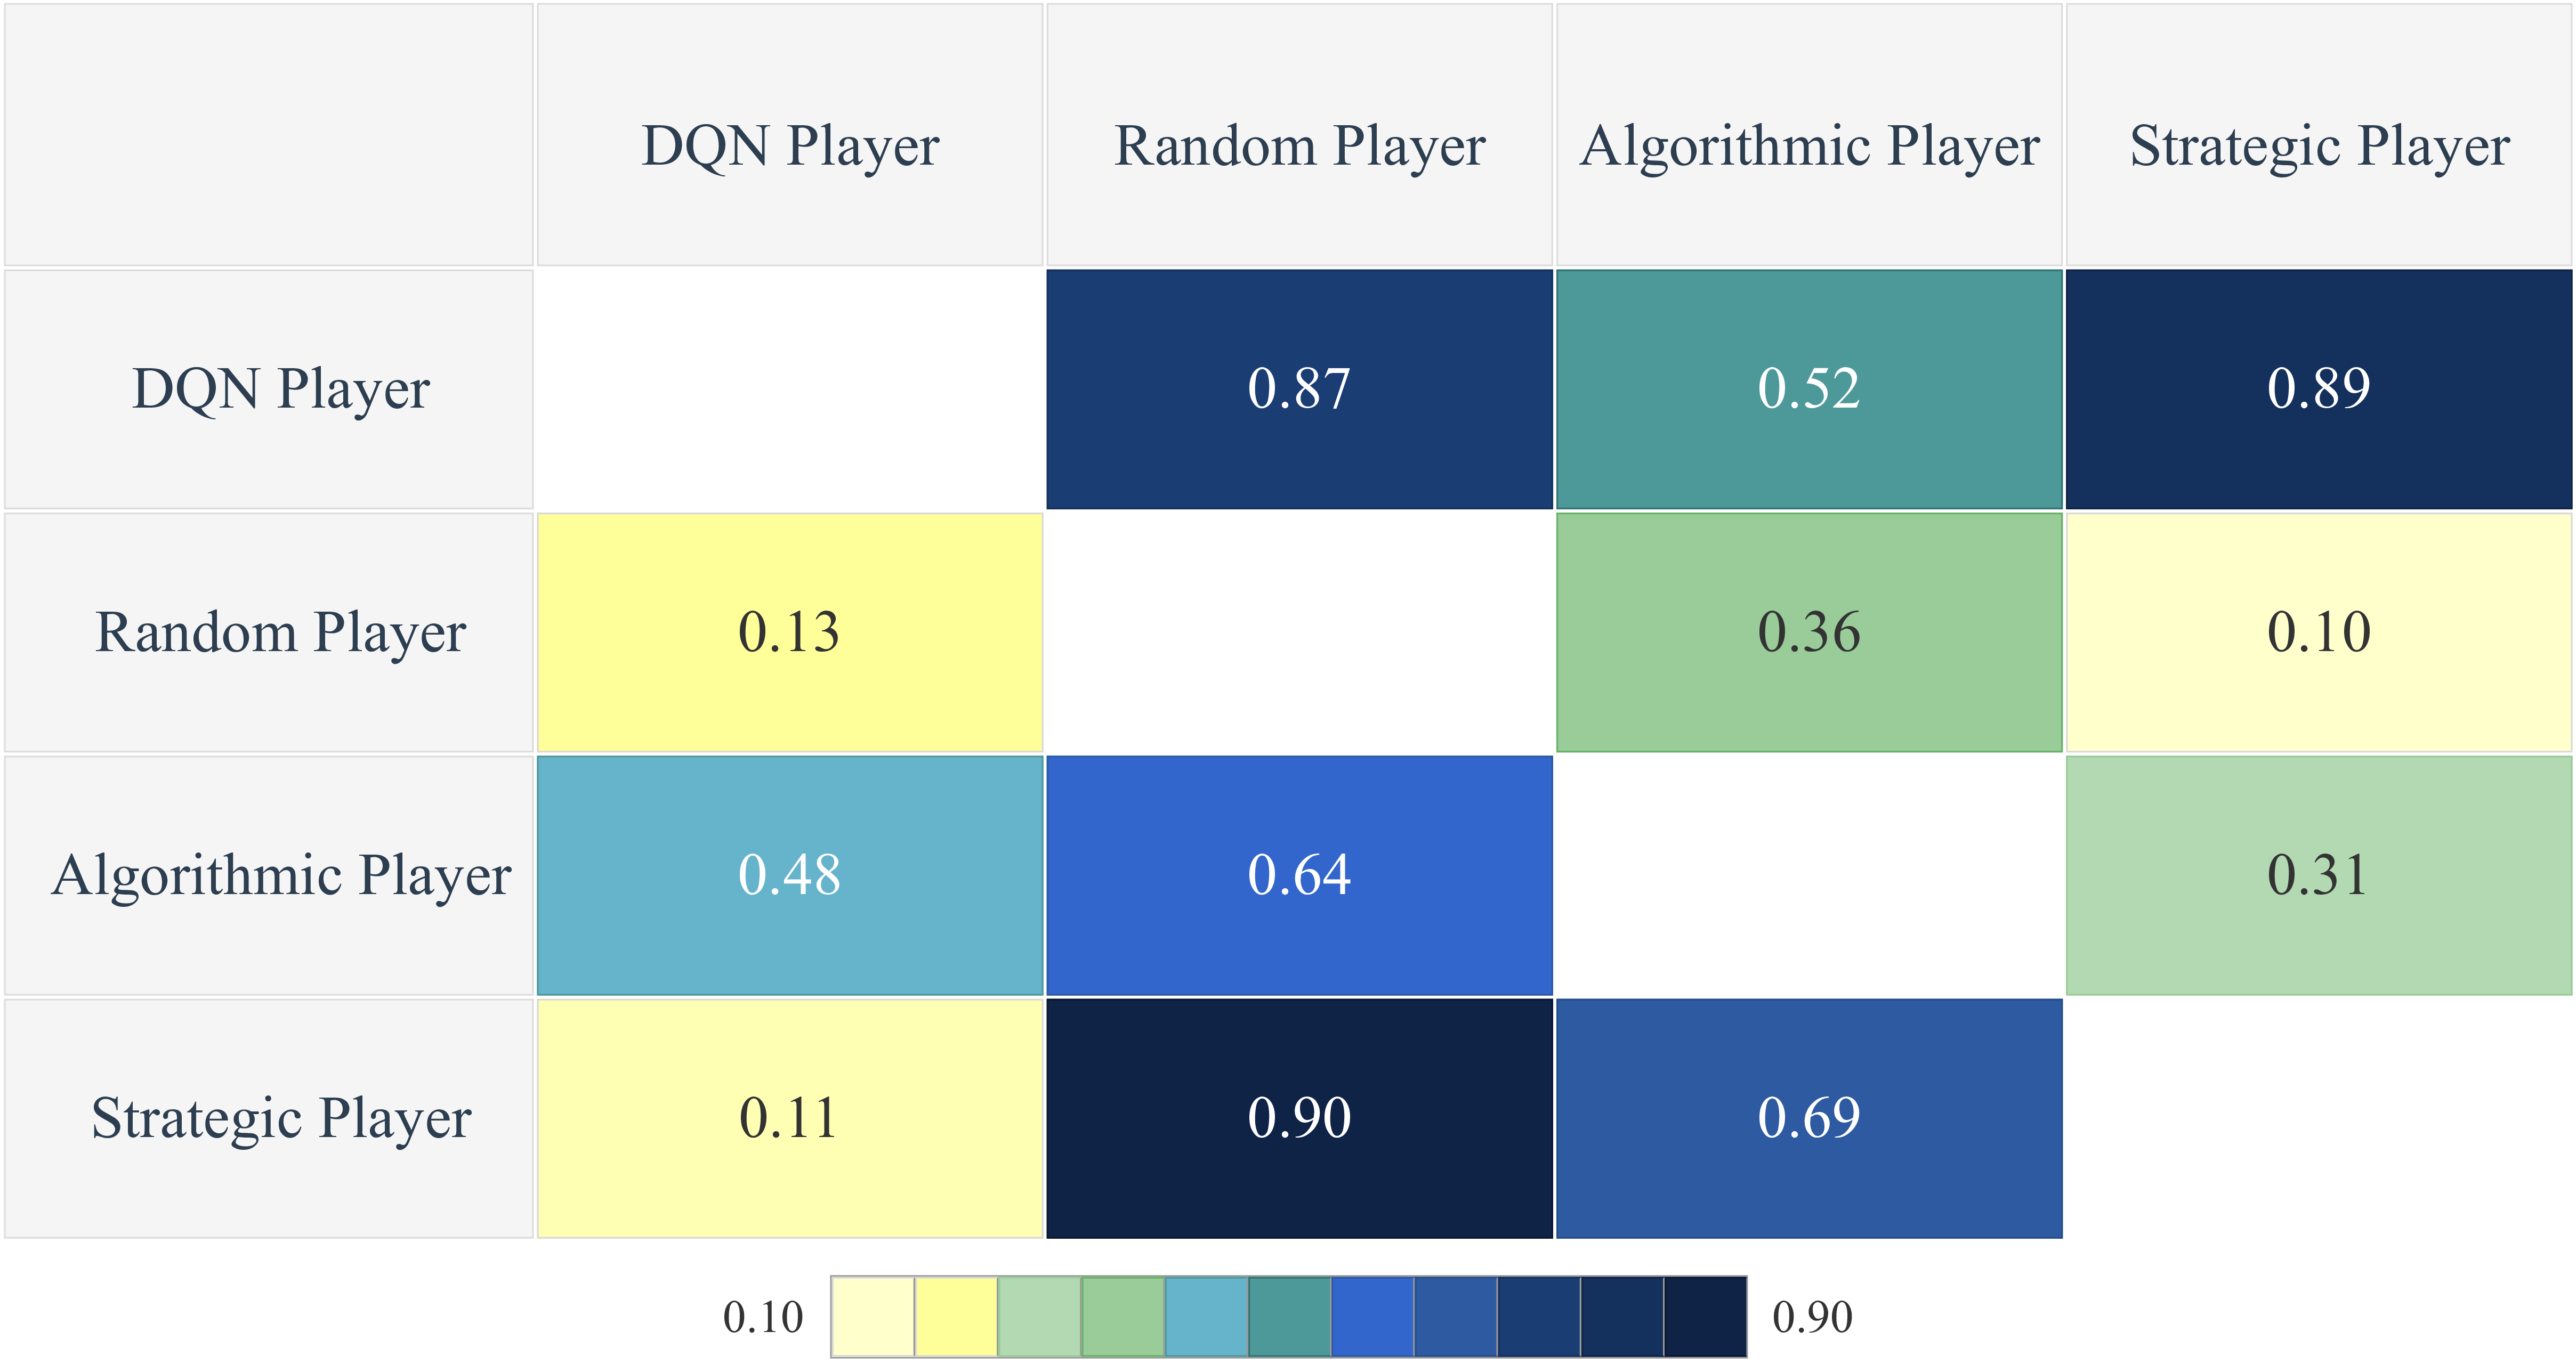
\includegraphics[width=13cm]{images/mini-tournament-dqn.png}
    \caption{Rezultatul turneului cu număr restrâns de agenți}
    \label{fig:mini-tournament-results}
\end{figure}

În cazul duelurilor cu agenții de bază, rezultatul fiind ilustrat în figura \ref{fig:mini-tournament-results}, agentul DQN pare să aibă probleme în înfrângerea celui algoritmic. O ipoteză în această privință poate consta în evitarea antrenamentelor împotriva sa, agentul algoritmic fiind folosit ca punct de "testare". Astfel, cum agentul DQN nu a fost antrenat împotriva sa, agentul algoritmic pare să introducă o strategie în fața căreia agentul DQN se poate adapta, dat fiind rezultatul de 51\% rată de câștig, dar pe care nu o poate înfrânge, dată fiind necunoscuta politică abordată.

Datorită introducerii unui eveniment neașteptat, putem oferi încă o concluzie folositoare, aceea că agentul nostru reușește să fie și robust. Într-adevăr în cazul lucrărilor amintite anterior \cite{mdp_monopoly_2}, \cite{hybrid_monopoly}, antrenamentul și testarea s-a realizat exclusiv pe baza acelorași agenți, astfel introducând un element de bias în structura decizională a agentului. Prin excluderea agentului algoritmic, am reușit să creăm o referință importantă în evaluarea sa, punct ce ne va ajuta să înțelegem cu adevărat puterea de adaptabilitate a agentului, în contextul dat, fiind una medie, reușind să depășească marja de egalitate.

\section{Dezvoltări ulterioare}
Alegerea algoritmului DQN pentru arhitectura agentului a fost inspirată din simplitatea și ușurința de implementare a acestuia, fiind baza în cadrul învățării adânci prin întărire. Deși minimalistă, această abordare poate fi mai slabă în contextul jocurilor complexe, preferându-se o variantă care învață o politică, în schimbul învățării valorilor Q.

Lucrarea \cite{hybrid_monopoly} folosește o optimizare proximală a politicii (Proximal Policy Optimization, PPO), care rezultă într-o rată de câștig comparativ mai mare față de o abordare a estimării valorii Q. Ca posibilitate de dezvoltare ulterioară aș încerca integrarea algoritmului A2C (Advantage Actor Critic), pentru observarea schimbării performanțelor și al politicii deprinse.

Aș încerca, de asemenea, modelarea și încorporarea funcției de schimb printr-un mecanism neuronal, astfel putând observa direct efectul acestora în parcursul jocului. Integrarea algoritmică nu favorizează o politică activă de schimb, ci doar o prezență pasivă în cadrul jocului, pentru a satisface nevoia de aprobare a unor schimburi existente.

\section{Aprecieri personale}
Consider că rezultatele obținute sunt satisfăcătoare și vor reprezenta un punct de plecare în considerentele viitoare. Abordarea descrisă este menită să încurajeze dezvoltări ulterioare și testări noi de teorii, oferind un sistem funcțional și scalabil.

Scopul lucrării a fost de actualizare a rezultatelor și concluzionare a unor lucrări existente, prin prisma dezvoltării unei noi abordări ușor de înțeles și de folosit.